\section{Desenho}
\tkzname{\tkznameofpack} pode desenhar 5 tipos de objetos: ponto, reta ou segmento de reta, círculo, arco e setor.

%<---------------------------------------------------------------------------->
%    POINT(S)
%<---------------------------------------------------------------------------->
\subsection{Desenhar um ponto ou alguns pontos}
Existem duas possibilidades: \tkzcname{tkzDrawPoint} para um único ponto ou \tkzcname{tkzDrawPoints} para um ou mais pontos.

\subsubsection{Desenhando pontos \tkzcname{tkzDrawPoint}} \hypertarget{tdrp}{}

\begin{NewMacroBox}{tkzDrawPoint}{\oarg{local opções}\parg{name}}%
\begin{tabular}{lll}%
argumentos &  padrão & definição                 \\
\midrule
\TAline{name of point} {sem padrão}  {Apenas um nome de ponto é aceito}
\bottomrule
\end{tabular}

\medskip
O argumento é obrigatório. O disco assume a cor do círculo, mas mais claro. É possível alterar tudo. O ponto é um nó e, portanto, é invariante se o desenho for modificado por escala.

\medskip
\begin{tabular}{lll}%
\toprule
opções             & padrão & definição \\
\midrule
\TOline{\TIKZ\ opções}{}{todas as opções \TIKZ\ são válidas.}
\TOline{shape}  {circle}{Possível \tkzname{cross} ou \tkzname{cross out}}
\TOline{size}   {6}{$6 \times$ \tkzcname{pgflinewidth}}
\TOline{color}  {black}{a cor padrão pode ser alterada}
\bottomrule
\end{tabular}

\medskip
{Podemos criar outras formas como \tkzname{cross}}
\end{NewMacroBox}

Por padrão, \tkzname{point style} é definido assim:

\begin{tkzltxexample}[]
  \tikzset{point style/.style = {%
           draw         = black,
           inner sep    = 0pt,
           shape        = circle,
           minimum size = 3 pt,
           fill         = black
                               }
        } 
\end{tkzltxexample}

\subsubsection{Exemplo de desenho de pontos}
Note que \tkzname{scale} não afeta a forma dos pontos. O que é normal. Na maioria das vezes, ficamos satisfeitos com uma única forma de ponto que podemos definir desde o início, seja com uma macro ou modificando um arquivo de configuração.

\begin{tkzexample}[latex=5cm,small]
  \begin{tikzpicture}[scale=.5]
   \tkzDefPoint(1,3){A}
   \tkzDefPoint(4,1){B}
   \tkzDefPoint(0,0){O}
   \tkzDrawPoint[color=red](A)
   \tkzDrawPoint[fill=blue!20,draw=blue](B)
   \tkzDrawPoint[shape=cross,size=8pt,color=teal](O)
  \end{tikzpicture}
\end{tkzexample}

É possível desenhar vários pontos de uma só vez, mas esta macro é um pouco mais lenta que a anterior. Além disso, temos que nos contentar com as mesmas opções para todos os pontos.
\newpage
\hypertarget{tdrps}{}
\begin{NewMacroBox}{tkzDrawPoints}{\oarg{local opções}\parg{liste}}%
\begin{tabular}{lll}%
argumentos &  padrão  & definição \\
\midrule
\TAline{points list}{sem padrão}{exemplo \tkzcname{tkzDrawPoints(A,B,C)}}
\bottomrule
\end{tabular}

\medskip
\begin{tabular}{lll}%
opções             & padrão & definição \\
\midrule
\TOline{shape}  {circle}{Possível \tkzname{cross} ou \tkzname{cross out}}
\TOline{size}  {6}{$6 \times$ \tkzcname{pgflinewidth}}
\TOline{color}  {black}{a cor padrão pode ser alterada}
\bottomrule
\end{tabular}

\medskip
\tkzHandBomb\ Cuidado com o \code{s} final, um descuido leva a erros em cascata se você tentar desenhar vários pontos. As opções são as mesmas da macro anterior.
\end{NewMacroBox}

\subsubsection{Exemplo}

\begin{tkzexample}[latex=7cm,small]
\begin{tikzpicture}
\tkzDefPoints{1/3/A,4/1/B,0/0/C}
\tkzDrawPoints[size=3,color=red,fill=red!50](A,B,C)
\end{tikzpicture}
\end{tkzexample}
%<---------------------------------------------------------------------------->
%    LINE(S)
%<---------------------------------------------------------------------------->
\section{Desenhando as retas}
As macros seguintes são simplesmente usadas para desenhar e nomear retas.
\subsection{Desenhar uma reta}
Para desenhar uma reta normal, basta fornecer um par de pontos. Você pode usar a opção \tkzname{add} para estender a reta (Esta opção é devida a \tkzimp{Mark Wibrow}, veja o código abaixo).

O estilo de uma reta é por padrão:

\begin{tkzltxexample}[]
  \tikzset{line style/.style = {%
    line width = 0.6pt,
    color      = black,
    style      = solid,
    add        = {.2} and  {.2}%
   }}
\end{tkzltxexample}
with
   
\begin{tkzltxexample}[]
  \tikzset{%
    add/.style args={#1 and #2}{
        to path={%
 ($(\tikztostart)!-#1!(\tikztotarget)$)--($(\tikztotarget)!-#2!(\tikztostart)$)%
  \tikztonodes}}}
\end{tkzltxexample}

Você pode modificar este estilo com \tkzcname{tkzSetUpLine} veja \ref{tkzsetupline}

\newpage
\begin{NewMacroBox}{tkzDrawLine}{\oarg{local opções}\parg{pt1,pt2} }%
Os argumentos são uma lista de dois ou três pontos. Seria possível, como para uma semirreta, criar um estilo com \tkzcname{add}.

\begin{tabular}{lll}%
\toprule
opções             & padrão & definição                         \\
\midrule
\TOline{\TIKZ\ opções}{}{todas as opções \TIKZ\ são válidas.}
\TOline{add}{0.2 and 0.2}{add = $kl$ and $kr$, \dots}
\TOline{\dots}{\dots}{permite que o segmento seja estendido para a esquerda e direita.}
\bottomrule
\end{tabular}

\tkzname{add} define o comprimento da reta passando pelos pontos pt1 e pt2. Ambos os números são percentagens. Os estilos do \TIKZ\ estão acessíveis para os desenhos.
\end{NewMacroBox}

\subsubsection{Exemplos  with \tkzname{add}}
\begin{tkzexample}[latex=5cm,small]
\begin{tikzpicture}
 \tkzInit[xmin=-2,xmax=3,ymin=-2.25,ymax=2.25]
 \tkzClip[space=.25]
 \tkzDefPoint(0,0){A} \tkzDefPoint(2,0.5){B}
 \tkzDefPoint(0,-1){C}\tkzDefPoint(2,-0.5){D} 
 \tkzDefPoint(0,1){E} \tkzDefPoint(2,1.5){F} 
 \tkzDefPoint(0,-2){G} \tkzDefPoint(2,-1.5){H}
 \tkzDrawLine(A,B)    \tkzDrawLine[add = 0 and .5](C,D) 
 \tkzDrawLine[add = 1 and 0](E,F)
 \tkzDrawLine[add = 0 and 0](G,H) 
 \tkzDrawPoints(A,B,C,D,E,F,G,H)    
 \tkzLabelPoints(A,B,C,D,E,F,G,H)  
\end{tikzpicture}
\end{tkzexample} 

É possível desenhar várias retas, mas com as mesmas opções.
\begin{NewMacroBox}{tkzDrawLines}{\oarg{local opções}\parg{pt1,pt2 pt3,pt4 ...}}%
Os argumentos são uma lista de pares de pontos separados por espaços. Os estilos do \TIKZ\ estão disponíveis para os desenhos.
\end{NewMacroBox}      

\subsubsection{Exemplo with \tkzcname{tkzDrawLines}}    

\begin{tkzexample}[latex=8cm,small]
\begin{tikzpicture}
  \tkzDefPoint(0,0){A}
  \tkzDefPoint(2,0){B}
  \tkzDefPoint(1,2){C}
  \tkzDefPoint(3,2){D}   
  \tkzDrawLines(A,B C,D A,C B,D)
  \tkzLabelPoints(A,B,C,D)
\end{tikzpicture}
\end{tkzexample}
%<---------------------------------------------------------------------------->
%    SEGMENT(S)
%<---------------------------------------------------------------------------->
\section{Desenhando um segmento}
Há, é claro, uma macro para simplesmente desenhar um segmento.

\subsection{Desenhar um segmento \tkzcname{tkzDrawSegment}}
\begin{NewMacroBox}{tkzDrawSegment}{\oarg{local opções}\parg{pt1,pt2}}%
Os argumentos são uma lista de dois pontos. Os estilos do \TIKZ\ estão disponíveis para os desenhos.
 
\medskip
\begin{tabular}{lll}%
argument    & exemplo & definição    \\
\midrule
\TAline{(pt1,pt2)}{(A,B)}{desenha o segmento $[A,B]$}
\bottomrule 
\end{tabular}
 
\medskip
\begin{tabular}{lll}%
opções    & exemplo & definição    \\
\midrule
\TOline{\TIKZ\ opções}{}{todas as opções \TIKZ\ são válidas.}
\TOline{dim}{sem padrão}{dim = \{label,dim,opção\}, \dots}
\TOline{\dots}{\dots}{permite adicionar dimensões a uma figura.}
\bottomrule
\end{tabular}

Isso é, claro, equivalente a \tkzcname{draw (A)--(B);}. Você também pode usar a opção \tkzname{add}.
\end{NewMacroBox}

\subsubsection{Exemplo com referências de pontos}     

\begin{tkzexample}[latex=6cm,small]
\begin{tikzpicture}[scale=1.5]
  \tkzDefPoint(0,0){A}
  \tkzDefPoint(2,1){B}
  \tkzDrawSegment[color=red,thin](A,B)
  \tkzDrawPoints(A,B)    
  \tkzLabelPoints(A,B)  
\end{tikzpicture}
\end{tkzexample}

\subsubsection{Exemplo de extensão de um segmento com opção \tkzname{add}} 

\begin{tkzexample}[latex=7cm,small]
\begin{tikzpicture}
  \tkzDefPoints{0/0/A,6/0/B,0.8/4/C}
  \tkzDefTriangleCenter[euler](A,B,C) 
  \tkzGetPoint{E}
  \tkzDefCircle[euler](A,B,C)\tkzGetPoints{E}{e}
  \tkzDrawCircle[red](E,e)
  \tkzDrawLines[add=.5 and .5](A,B A,C B,C)
  \tkzDrawPoints(A,B,C,E)
  \tkzLabelPoints(A,B,C,E)
  \end{tikzpicture}
\end{tkzexample}

\subsubsection{Adicionando dimensões com opção \tkzname{dim} novo código de Muzimuzhi Z}
Este código vem de uma resposta a esta pergunta no tex.stackexchange.com
(change-color-and-style-of-dimension-lines-in-tkz-euclide ).
O código do \tkzname{dim} é baseado em opções do TikZ, você deve adicionar as unidades.
Você pode usar agora dois estilos: |dim style| e |dim fence style|. Você tem várias maneiras de usá-los.
Vou deixar você olhar os exemplos para ver o que pode fazer com esses estilos.

\begin{verbatim}
   \tikzset{dim style/.append style={dashed}} % append if you want to keep precedent style.
   or 
   \begin{scope}[ dim style/.append style={orange},
       dim fence style/.style={dashed}]
\end{verbatim}

\begin{tkzexample}[latex=7cm]
\begin{tikzpicture}[scale=.75]
  \tkzDefPoints{0/3/A, 1/-3/B}
  \tkzDrawPoints(A,B)
  \tkzDrawSegment[dim={\(l_0\),1cm,right=2mm}, 
    dim style/.append style={red, 
    dash pattern={on 2pt off 2pt}}](A,B)
  \tkzDrawSegment[dim={\(l_1\),2cm,right=2mm}, 
    dim style/.append style={blue}](A,B)
  \begin{scope}[ dim style/.style={orange},
      dim fence style/.style={dashed}]
    \tkzDrawSegment[dim={\(l_2\),3cm,right=2mm}](A,B)  
    \tkzDrawSegment[dim={\(l_3\),-2cm,right=2mm}](A,B)   
  \end{scope}  
  \tkzLabelPoints[left](A,B)
\end{tikzpicture}
\end{tkzexample}

\subsubsection{Adicionando dimensões com opção \tkzname{dim} parte I} 
\begin{tkzexample}[latex=7cm,small]
\begin{tikzpicture}[scale=2]
\pgfkeys{/pgf/number format/.cd,fixed,precision=2}
\tkzDefPoint(0,0){A}
\tkzDefPoint(3.07,0){B}
\tkzInterCC[R](A,2.37)(B,1.82)
\tkzGetPoints{C}{C'}
\tkzDefCircle[in](A,B,C) \tkzGetPoints{G}{g}
\tkzDrawCircle(G,g)
\tkzDrawPolygon(A,B,C)
\tkzDrawPoints(A,B,C)
\tkzCalcLength(A,B)\tkzGetLength{ABl}
\tkzCalcLength(B,C)\tkzGetLength{BCl}
\tkzCalcLength(A,C)\tkzGetLength{ACl}
\begin{scope}[dim style/.style={dashed,sloped,teal}]
  \tkzDrawSegment[dim={\pgfmathprintnumber\BCl,6pt,%
                                      text=red}](C,B)
  \tkzDrawSegment[dim={\pgfmathprintnumber\ACl,%
                                        6pt,}](A,C)
  \tkzDrawSegment[dim={\pgfmathprintnumber\ABl,%
                                      -6pt,}](A,B)
\end{scope}
\tkzLabelPoints(A,B) \tkzLabelPoints[above](C)
\end{tikzpicture}
\end{tkzexample}

\subsubsection{Adicionando dimensões com opção \tkzname{dim} parte II} 
\begin{tkzexample}[latex=6cm,small]
\begin{tikzpicture}[scale=.5]
  \tkzDefPoints{0/0/O,-2/0/A,2/0/B,
                -2/4/C,2/4/D,2/-4/E,-2/-4/F}
  \tkzDrawPolygon(C,...,F)
  \tkzDrawSegments(A,B)
  \tkzDrawPoints(A,...,F,O)
  \tkzLabelPoints[below left](A,...,F,O)
  \tkzDrawSegment[dim={ $\sqrt{5}$,2cm,}](C,E)
  \tkzDrawSegment[dim={ $\frac{\sqrt{5}}{2}$,1cm,}](O,E)
  \tkzDrawSegment[dim={ $2$,2cm,left=8pt}](F,C)
  \tkzDrawSegment[dim={ $1$,1cm,left=8pt}](F,A)
\end{tikzpicture}
\end{tkzexample}

\subsection{Desenhando segmentos \tkzcname{tkzDrawSegments}}
Se as opções são as mesmas, podemos desenhar vários segmentos com a mesma macro.

\begin{NewMacroBox}{tkzDrawSegments}{\oarg{local opções}\parg{pt1,pt2 pt3,pt4 ...}}%
Os argumentos são uma lista de pares de pontos. Os estilos do \TIKZ\ estão disponíveis para os desenhos.
\end{NewMacroBox}

\begin{tkzexample}[latex=6cm,small]
\begin{tikzpicture}
  \tkzInit[xmin=-1,xmax=3,ymin=-1,ymax=2]
  \tkzClip[space=1]
  \tkzDefPoint(0,0){A}
  \tkzDefPoint(2,1){B} 
  \tkzDefPoint(3,0){C} 
  \tkzDrawSegments(A,B B,C)
  \tkzDrawPoints(A,B,C)    
  \tkzLabelPoints(A,C) 
  \tkzLabelPoints[above](B)  
\end{tikzpicture}
\end{tkzexample}

\subsubsection{Colocar uma seta em um segmento}
\begin{tkzexample}[latex=6cm,small]
\begin{tikzpicture}
\tkzSetUpStyle[postaction=decorate,
    decoration={markings, 
    mark=at position .5 with {\arrow[thick]{#1}}
      }]{myarrow}
  \tkzDefPoint(0,0){A}
  \tkzDefPoint(4,-4){B}
  \tkzDrawSegments[myarrow=stealth](A,B)
  \tkzDrawPoints(A,B) 
\end{tikzpicture}
\end{tkzexample}

\subsection{Desenhando segmentos de reta de um triângulo}

\subsubsection{Como desenhar \tkzname{Altitude}} 
\begin{tkzexample}[latex=7cm,small]
  \begin{tikzpicture}[rotate=-90]
  \tkzDefPoint(0,1){A}
  \tkzDefPoint(2,4){C}
  \tkzDefPointWith[orthogonal normed,K=7](C,A)
  \tkzGetPoint{B}
  \tkzDefSpcTriangle[orthic,name=H](A,B,C){a,b,c}
  \tkzDrawLine[dashed,color=magenta](C,Hc)
  \tkzDrawSegment[green!60!black](A,C)
  \tkzDrawSegment[green!60!black](C,B)
  \tkzDrawSegment[green!60!black](B,A)
  \tkzLabelPoint[left](A){$A$}
  \tkzLabelPoint[right](B){$B$}
  \tkzLabelPoint[above](C){$C$}
  \tkzLabelPoint[left](Hc){$Hc$}
  \tkzLabelSegment[auto](B,A){$c$}
  \tkzLabelSegment[auto,swap](B,C){$a$}
  \tkzLabelSegment[auto,swap](C,A){$b$}
  \tkzMarkAngle[size=1,color=cyan,mark=|](C,B,A)
  \tkzMarkAngle[size=1,color=cyan,mark=|](A,C,Hc)
  \tkzMarkAngle[size=0.75,
                color=orange,mark=||](Hc,C,B)
  \tkzMarkAngle[size=0.75,
                color=orange,mark=||](B,A,C)
  \tkzMarkRightAngle(A,C,B)
  \tkzMarkRightAngle(B,Hc,C)
  \end{tikzpicture} 
\end{tkzexample}

\subsection{Desenhando um polígono}
 \begin{NewMacroBox}{tkzDrawPolygon}{\oarg{local opções}\parg{points list}}%
Basta fornecer uma lista de pontos e a macro desenha o polígono usando as opções \TIKZ\ presentes. Você pode substituir $(A,B,C,D,E)$ por $(A,...,E)$ e $(P_1,P_2,P_3,P_4,P_5)$ por $(P_1,P...,P_5)$

\begin{tabular}{lll}%
\toprule
argumentos             & exemplo & explicação                         \\
\midrule
\TAline{\parg{pt1,pt2,pt3,...}}{|\BS tkzDrawPolygon[gray,dashed](A,B,C)|}{Desenhando um triângulo}
\end{tabular}

\medskip
\begin{tabular}{lll}%
\toprule
opções             & padrão & exemplo                         \\
\midrule
\TOline{Opções TikZ}{...}{|\BS tkzDrawPolygon[red,line width=2pt](A,B,C)|}
 \end{tabular}
\end{NewMacroBox}

\subsubsection{\tkzcname{tkzDrawPolygon}}

\begin{tkzexample}[latex=7cm, small]  
\begin{tikzpicture} [rotate=18,scale=1]
 \tkzDefPoints{0/0/A,2.25/0.2/B,2.5/2.75/C,-0.75/2/D}
 \tkzDrawPolygon(A,B,C,D)
 \tkzDrawSegments[style=dashed](A,C B,D) 
\end{tikzpicture}
\end{tkzexample}

\subsubsection{Opção \tkzname{two angles}}
\begin{tkzexample}[latex=6 cm,small]
\begin{tikzpicture}
\tkzDefPoint(0,0){A} 
\tkzDefPoint(6,0){B} 
\tkzDefTriangle[two angles = 50 and 70](A,B) \tkzGetPoint{C}
\tkzDrawPolygon(A,B,C)
\tkzLabelAngle[pos=1.4](B,A,C){$50^\circ$}
\tkzLabelAngle[pos=0.8](C,B,A){$70^\circ$}
\end{tikzpicture}
\end{tkzexample}

\subsubsection{Estilo de linha}
\begin{tkzexample}[latex=8 cm,small]
\begin{tikzpicture}[scale=.6]
\tkzSetUpLine[line width=5mm,color=teal]
\tkzDefPoint(0,0){O}
\foreach \i in {0,...,5}{%
 \tkzDefPoint({30+60*\i}:4){p\i}}
\tkzDefMidPoint(p1,p3) \tkzGetPoint{m1}
\tkzDefMidPoint(p3,p5) \tkzGetPoint{m3}
\tkzDefMidPoint(p5,p1) \tkzGetPoint{m5}
\tkzDrawPolygon[line join=round](p1,p3,p5)
\tkzDrawPolygon[teal!80,
line join=round](p0,p2,p4)
\tkzDrawSegments(m1,p3 m3,p5 m5,p1)
\tkzDefCircle[R](O,4.8)\tkzGetPoint{o}
\tkzDrawCircle[teal](O,o)
\end{tikzpicture}
\end{tkzexample}

\subsection{Desenhando uma cadeia poligonal}
 \begin{NewMacroBox}{tkzDrawPolySeg}{\oarg{local opções}\parg{points list}}%
Basta fornecer uma lista de pontos e a macro desenha a cadeia poligonal usando as opções \TIKZ\ presentes.

\begin{tabular}{lll}%
\toprule
argumentos             & exemplo & explicação                         \\
\midrule
\TAline{\parg{pt1,pt2,pt3,...}}{|\BS tkzDrawPolySeg[gray,dashed](A,B,C)|}{Desenhando um triângulo}
\end{tabular}

\medskip
\begin{tabular}{lll}%
\toprule
opções             & padrão & exemplo                         \\
\midrule
\TOline{Opções TikZ}{...}{|\BS tkzDrawPolySeg[red,line width=2pt](A,B,C)|}
 \end{tabular}
\end{NewMacroBox}

\subsubsection{Cadeia poligonal}

\begin{tkzexample}[latex=7cm, small]  
\begin{tikzpicture}
 \tkzDefPoints{0/0/A,6/0/B,3/4/C,2/2/D}          
 \tkzDrawPolySeg(A,...,D)
 \tkzDrawPoints(A,...,D)
\end{tikzpicture}
\end{tkzexample}

\subsubsection{A ideia é inscrever dois quadrados em um semicírculo.}
Um visual Sangaku! Trata-se de provar que se pode inscrever em um meio disco, dois quadrados, e determinar o comprimento de seus respectivos lados de acordo com o raio.

\begin{tkzexample}[latex=7 cm,small]
\begin{tikzpicture}[scale=.75] 
  \tkzDefPoints{0/0/A,8/0/B,4/0/I}
  \tkzDefSquare(A,B)    \tkzGetPoints{C}{D} 
  \tkzInterLC(I,C)(I,B) \tkzGetPoints{E'}{E} 
  \tkzInterLC(I,D)(I,B) \tkzGetPoints{F'}{F} 
  \tkzDefPointsBy[projection=onto A--B](E,F){H,G} 
  \tkzDefPointsBy[symmetry = center H](I){J} 
  \tkzDefSquare(H,J)     \tkzGetPoints{K}{L} 
  \tkzDrawSector(I,B)(A) 
  \tkzDrawPolySeg(H,E,F,G) 
  \tkzDrawPolySeg(J,K,L) 
  \tkzDrawPoints(E,G,H,F,J,K,L)
\end{tikzpicture}
\end{tkzexample}

\subsubsection{Cadeia poligonal: notação de índice}

\begin{tkzexample}[latex=7cm, small]  
\begin{tikzpicture}
\foreach \pt in {1,2,...,8} {%
\tkzDefPoint(\pt*20:3){P_\pt}}     
\tkzDrawPolySeg(P_1,P_...,P_8)
\tkzDrawPoints(P_1,P_...,P_8)
\end{tikzpicture}
\end{tkzexample}
%<---------------------------------------------------------------------------->
%    CIRCLE
%<---------------------------------------------------------------------------->
\section{Desenhar um círculo com \tkzcname{tkzDrawCircle}}

\subsection{Desenhar um círculo}
\begin{NewMacroBox}{tkzDrawCircle}{\oarg{local opções}\parg{A,B}}%
\tkzHandBomb\ Atenção, você precisa apenas de dois pontos para definir um raio. Uma opção adicional \tkzname{R} está disponível para fornecer uma medida diretamente.

\medskip
\begin{tabular}{lll}%
\toprule
argumentos           & exemplo & explicação                         \\
\midrule
\TAline{\parg{pt1,pt2}}{\parg{A,B}} {A centro passando por B}
 \bottomrule
\end{tabular}

\medskip
Claro, você tem que adicionar todos os estilos do \TIKZ\ para os traçados...
\end{NewMacroBox}

 \subsubsection{Círculos e estilos, desenhar um círculo e colorir o disco}
 Veremos que é possível colorir um disco enquanto se traça o círculo.
 
\begin{tkzexample}[latex=7cm,small]
\begin{tikzpicture}
  \tkzDefPoint(0,0){O} 
  \tkzDefPoint(3,0){A}
 % circle with center O and passing through A
  \tkzDrawCircle(O,A) 
 % diameter circle $[OA]$
 \tkzDefCircle[diameter](O,A) \tkzGetPoint{I}
 \tkzDrawCircle[new,fill=orange!10,opacity=.5](I,A)
 % circle with center O and radius = exp(1) cm
  \edef\rayon{\fpeval{0.25*exp(1)}}
  \tkzDefCircle[R](O,\rayon) \tkzGetPoint{o}
   \tkzDrawCircle[color=orange](O,o) 
\end{tikzpicture} 
\end{tkzexample}  

\subsection{Desenhando círculos}
\begin{NewMacroBox}{tkzDrawCircles}{\oarg{local opções}\parg{A,B C,D \dots}}%
\tkzHandBomb\ Atenção, os argumentos são listas de dois pontos. Os círculos que podem ser desenhados são os mesmos da macro anterior. Uma opção adicional \tkzname{R} está disponível para fornecer uma medida diretamente.

\medskip
\begin{tabular}{lll}%
\toprule
argumentos           & exemplo & explicação                         \\
\midrule
\TAline{\parg{pt1,pt2 pt3,pt4 ...}}{\parg{A,B C,D}} {Lista de dois pontos}
\bottomrule
\end{tabular}

\medskip
\begin{tabular}{lll}%
\toprule
opções             & padrão & definição                         \\
\midrule
\TOline{through}{through}{círculo com dois pontos definindo um raio}
 \bottomrule
\end{tabular}

\medskip
Você não precisa usar a opção padrão \tkzname{through}.
Claro, você tem que adicionar todos os estilos do \TIKZ\ para os traçados...
\end{NewMacroBox}

 \subsubsection{Círculos definidos por um triângulo.} 
 
\begin{tkzexample}[latex=9cm,small]
\begin{tikzpicture}
  \tkzDefPoints{0/0/A,2/0/B,3/2/C}
  \tkzDrawPolygon(A,B,C)
  \tkzDrawCircles(A,B B,C C,A)
  \tkzDrawPoints(A,B,C)
  \tkzLabelPoints(A,B,C) 
\end{tikzpicture} 
\end{tkzexample}

\subsubsection{Círculos concêntricos.} 
 
\begin{tkzexample}[latex=7cm,small]
\begin{tikzpicture}
   \tkzDefPoints{0/0/A,1/0/a,2/0/b,3/0/c}
   \tkzDrawCircles(A,a A,b A,c)
   \tkzDrawPoint(A)
   \tkzLabelPoints(A)
\end{tikzpicture}
\end{tkzexample}

\subsubsection{Círculos ex-inscritos.} 

\begin{tkzexample}[latex=8cm,small] 
\begin{tikzpicture}[scale=1] 
\tkzDefPoints{0/0/A,4/0/B,1/2.5/C}
\tkzDrawPolygon(A,B,C)
\tkzDefCircle[ex](B,C,A) 
\tkzGetPoint{J_c} \tkzGetSecondPoint{T_c}
\tkzDrawCircle(J_c,T_c)
\tkzDrawLines[add=0 and 1](C,A C,B)
\tkzDrawSegment(J_c,T_c)
\tkzMarkRightAngle(J_c,T_c,B)
\tkzDrawPoints(A,B,C,J_c,T_c)
\end{tikzpicture}
\end{tkzexample}
 
\subsubsection{Cardioide}
Baseado em uma ideia de O. Reboux feita com pst-eucl (módulo Pstricks) por D. Rodriguez.

 Seu nome vem do grego \textit{kardia (coração)}, em referência à sua forma, e foi dado a ela por Johan Castillon (Wikipedia).     
 
\begin{tkzexample}[latex=7cm,small]
\begin{tikzpicture}[scale=.5]
  \tkzDefPoint(0,0){O} 
  \tkzDefPoint(2,0){A}
  \foreach \ang in {5,10,...,360}{%
     \tkzDefPoint(\ang:2){M}
     \tkzDrawCircle(M,A) 
   }  
\end{tikzpicture} 
\end{tkzexample}

\newpage

\subsection{Desenhando semicírculo}
\begin{NewMacroBox}{tkzDrawSemiCircle}{\oarg{local opções}\parg{O,A}}%

\medskip
\begin{tabular}{lll}%
\toprule
argumentos           & exemplo & explicação                         \\
\midrule
\TAline{\parg{pt1,pt2}}{\parg{O,A}} {OA= raio}
\bottomrule
\end{tabular}

$O$ centro $A$ extremidade do semicírculo
\end{NewMacroBox}

\subsubsection{Uso de \tkzcname{tkzDrawSemiCircle}}   

\begin{tkzexample}[latex=7cm,small]
\begin{tikzpicture}
   \tkzDefPoint(0,0){A} \tkzDefPoint(6,0){B}
   \tkzDefMidPoint(A,B)  \tkzGetPoint{O}
   \tkzDrawSemiCircle[blue](O,B)
   \tkzDrawSemiCircle[red](O,A)
   \tkzDrawPoints(O,A,B)
   \tkzLabelPoints[below right](O,A,B)
 \end{tikzpicture}
\end{tkzexample}

\subsection{Desenhando semicírculos}

\begin{NewMacroBox}{tkzDrawSemiCircles}{\oarg{local opções}\parg{A,B C,D \dots}}%

\medskip
\begin{tabular}{lll}%
\toprule
argumentos           & exemplo & explicação                         \\
\midrule
\TAline{\parg{pt1,pt2 pt3,pt4 ...}}{\parg{A,B C,D}} {Lista de dois pontos}
\bottomrule
\end{tabular}

\end{NewMacroBox}

\subsubsection{Uso de \tkzcname{tkzDrawSemiCircles} : Arbelos dourado}  

\begin{tkzexample}[vbox,small]
\begin{tikzpicture}[scale=.75]
\tkzDefPoints{0/0/A,10/0/B}
\tkzDefGoldenRatio(A,B) \tkzGetPoint{C}
\tkzDefMidPoint(A,B)                     \tkzGetPoint{O_0}
\tkzDefMidPoint(A,C)                     \tkzGetPoint{O_1}
\tkzDefMidPoint(C,B)                     \tkzGetPoint{O_2}
\tkzLabelPoints(A,B,C)
\tkzDrawSegment(A,B)
\tkzDrawPoints(A,B,C)
\begin{scope}[local bounding box = graph]
  \tkzDrawSemiCircles[color=black](O_0,B)
\end{scope}
\useasboundingbox (graph.south west) rectangle (graph.north east);
\tkzClipCircle[out](O_1,C)\tkzClipCircle[out](O_2,B)
\tkzDrawSemiCircles[draw=none,fill=teal!15](O_0,B)
\tkzDrawSemiCircles[color=black](O_1,C O_2,B)
\end{tikzpicture}
\end{tkzexample}

%<---------------------------------------------------------------------------->
%    Ellipse
%<---------------------------------------------------------------------------->
\section{Desenhar uma elipse com \tkzcname{tkzDrawEllipse}}

\subsection{Desenhar uma elipse}
\begin{NewMacroBox}{tkzDrawEllipse}{\oarg{local opções}\parg{C,a,b,An}}%


\medskip
\begin{tabular}{lll}%
\toprule
argumentos           & exemplo & explicação                         \\
\midrule
\TAline{\parg{C,a,b,An}}{\parg{C,4,2,45}} {C centro; 4 e 2 comprimentos dos semi-eixos} \\
 & & 45 inclinação do eixo principal  \\
 \bottomrule
\end{tabular}

\medskip
Claro, você tem que adicionar todos os estilos do \TIKZ\ para os traçados...
\end{NewMacroBox}

\subsubsection{Exemplo de desenho de uma elipse}
\begin{tkzexample}[latex=6cm,small]
   \begin{tikzpicture}[scale=.75]
      \tkzDefPoint(0,4){C}
      \tkzDrawEllipse[blue](C,4,2,45)
      \tkzLabelPoints(C)
   \end{tikzpicture}
\end{tkzexample}

%<---------------------------------------------------------------------------->
%    ARC
%<---------------------------------------------------------------------------->
\section{Desenhando arcos}
\subsection{Macro: \tkzcname{tkzDrawArc} }
\begin{NewMacroBox}{tkzDrawArc}{\oarg{local opções}\parg{O,\dots}\parg{\dots}}%
Esta macro traça o arco de centro $O$. Dependendo das opções, os argumentos diferem. Trata-se de determinar um ponto inicial e um ponto final. Ou o ponto inicial é dado, o que é mais simples, ou o raio do arco é dado. Neste último caso, é necessário ter dois ângulos. Ou os ângulos podem ser dados diretamente, ou nós associados ao centro podem ser dados para determiná-los. Os ângulos estão em graus.

\medskip
\begin{tabular}{lll}%
\toprule
opções             & padrão & definição                        \\ 
\midrule
\TOline{towards}{towards}{$O$ é o centro e o arco de $A$ a $(OB)$}
\TOline{rotate} {towards}{o arco começa de $A$ e o ângulo determina seu comprimento}
\TOline{R}{towards}{Damos o raio e dois ângulos}
\TOline{R with nodes}{towards}{Damos o raio e dois pontos}
\TOline{angles}{towards}{Damos o raio e dois pontos}
\TOline{delta}{0}{ângulo adicionado em cada lado}
\TOline{reverse}{false}{inversão do caminho do arco, interessante para inverter seta}
\bottomrule
\end{tabular}

\medskip
Claro, você tem que adicionar todos os estilos do \TIKZ\ para os traçados...

\medskip

\begin{tabular}{lll}%
\toprule
opções             & argumentos & exemplo                         \\ 
\midrule
\TOline{towards}{\parg{pt,pt}\parg{pt}}{\tkzcname{tkzDrawArc[delta=10](O,A)(B)}} 
\TOline{rotate} {\parg{pt,pt}\parg{an}}{\tkzcname{tkzDrawArc[rotate,color=red](O,A)(90)}}
\TOline{R}{\parg{pt,$r$}\parg{an,an}}{\tkzcname{tkzDrawArc[R](O,2)(30,90)}}
\TOline{R with nodes}{\parg{pt,$r$}\parg{pt,pt}}{\tkzcname{tkzDrawArc[R with nodes](O,2)(A,B)}}
\TOline{angles}{\parg{pt,pt}\parg{an,an}}{\tkzcname{tkzDrawArc[angles](O,A)(0,90)}}
\end{tabular}
\end{NewMacroBox}

Aqui estão alguns exemplos:

\subsubsection{Opção \tkzname{towards}}
É inútil colocar \tkzname{towards}. Neste primeiro exemplo, o arco começa de $A$ e vai para $B$. O arco indo de $B$ para $A$ é diferente. O saliente é obtido indo na direção direta do círculo trigonométrico.
\begin{tkzexample}[latex=6cm,small]
\begin{tikzpicture}[scale=.75]
  \tkzDefPoint(0,0){O}
  \tkzDefPoint(2,-1){A}
  \tkzDefPointBy[rotation= center O angle 90](A)
  \tkzGetPoint{B}
  \tkzDrawArc[color=orange,<->](O,A)(B) 
  \tkzDrawArc(O,B)(A)
  \tkzDrawLines[add = 0 and .5](O,A O,B)
  \tkzDrawPoints(O,A,B)
  \tkzLabelPoints[below](O,A,B)  
\end{tikzpicture}
\end{tkzexample}

\subsubsection{Opção \tkzname{towards}}
Neste, o arco começa de A mas para na reta (OB).
 
\begin{tkzexample}[latex=6cm,small]
\begin{tikzpicture}[scale=0.75] 
  \tkzDefPoint(0,0){O}
  \tkzDefPoint(2,-1){A}
  \tkzDefPoint(1,1){B} 
  \tkzDrawArc[color=blue,->](O,A)(B)
  \tkzDrawArc[color=gray](O,B)(A)
  \tkzDrawArc(O,B)(A)
  \tkzDrawLines[add = 0 and .5](O,A O,B) 
  \tkzDrawPoints(O,A,B)
  \tkzLabelPoints[below](O,A,B)  
\end{tikzpicture}
\end{tkzexample}

\subsubsection{Opção \tkzname{rotate}}
\begin{tkzexample}[latex=6cm,small] 
\begin{tikzpicture}[scale=0.75] 
  \tkzDefPoint(0,0){O}
  \tkzDefPoint(2,-2){A}
  \tkzDefPoint(60:2){B}
  \tkzDrawLines[add = 0 and .5](O,A O,B)
  \tkzDrawArc[rotate,color=red](O,A)(180)
  \tkzDrawPoints(O,A,B)
  \tkzLabelPoints[below](O,A,B) 
\end{tikzpicture}
\end{tkzexample} 

\subsubsection{Opção \tkzname{R}} 
\begin{tkzexample}[latex=6cm,small]   
\begin{tikzpicture}[scale=0.75] 
  \tkzDefPoints{0/0/O}
  \tkzSetUpCompass[<->]
  \tkzDrawArc[R,color=teal,double](O,3)(270,360)
  \tkzDrawArc[R,color=orange,double](O,2)(0,270) 
  \tkzDrawPoint(O)
  \tkzLabelPoint[below](O){$O$}  
\end{tikzpicture} 
\end{tkzexample}

\subsubsection{Opção \tkzname{R with nodes}} 
\begin{tkzexample}[latex=6cm,small]
\begin{tikzpicture}[scale=0.75] 
  \tkzDefPoint(0,0){O}
  \tkzDefPoint(2,-1){A}
  \tkzDefPoint(1,1){B}
  \tkzCalcLength(B,A)\tkzGetLength{radius}
  \tkzDrawArc[R with nodes](B,\radius)(A,O)
\end{tikzpicture}
\end{tkzexample}

\subsubsection{Opção \tkzname{delta}}
Esta opção permite um pouco como \tkzcname{tkzCompass} colocar um arco e ultrapassar em cada lado. delta é uma medida em graus.

\begin{tkzexample}[latex=7cm,small] 
\begin{tikzpicture} 
 \tkzDefPoint(0,0){A}
 \tkzDefPoint(3,0){B}
 \tkzDefPointBy[rotation= center A angle 60](B)
 \tkzGetPoint{C} 
 \begin{scope}% style only local
   \tkzDefPointBy[symmetry= center C](A)
   \tkzGetPoint{D} 
   \tkzDrawSegments(A,B A,D)
   \tkzDrawLine(B,D)
   \tkzSetUpCompass[color=orange]
   \tkzDrawArc[orange,delta=10](A,B)(C)
   \tkzDrawArc[orange,delta=10](B,C)(A)
   \tkzDrawArc[orange,delta=10](C,D)(D)
 \end{scope}

 \tkzDrawPoints(A,B,C,D)
 \tkzLabelPoints[below right](A,B,C,D)
 \tkzMarkRightAngle(D,B,A)
\end{tikzpicture}
\end{tkzexample} 

\subsubsection{Opção \tkzname{angles}: exemplo 1}

\begin{tkzexample}[latex=6cm,small]
\begin{tikzpicture}[scale=.75]
  \tkzDefPoint(0,0){A}
  \tkzDefPoint(5,0){B}  
  \tkzDefPoint(2.5,0){O} 
  \tkzDefPointBy[rotation=center O angle 60](B)
  \tkzGetPoint{D}
  \tkzDefPointBy[symmetry=center D](O)
  \tkzGetPoint{E}
  \begin{scope}
    \tkzDrawArc[angles](O,B)(0,180)
    \tkzDrawArc[angles,](B,O)(100,180)  
    \tkzCompass[delta=20](D,E) 
    \tkzDrawLines(A,B O,E B,E)
    \tkzDrawPoints(A,B,O,D,E)
  \end{scope}
  \tkzLabelPoints[below right](A,B,O,D,E)
  \tkzMarkRightAngle(O,B,E) 
\end{tikzpicture} 
\end{tkzexample}

\subsubsection{Opção \tkzname{angles}: exemplo 2}

\begin{tkzexample}[latex=7cm,small]
  \begin{tikzpicture}
   \tkzDefPoint(0,0){O}
   \tkzDefPoint(5,0){I} 
   \tkzDefPoint(0,5){J}
   \tkzInterCC(O,I)(I,O)\tkzGetPoints{B}{C}  
   \tkzInterCC(O,I)(J,O)\tkzGetPoints{D}{A}
   \tkzInterCC(I,O)(J,O)\tkzGetPoints{L}{K}
   \tkzDrawArc[angles](O,I)(0,90)
   \tkzDrawArc[angles,color=gray,
               style=dashed](I,O)(90,180)
   \tkzDrawArc[angles,color=gray,
               style=dashed](J,O)(-90,0)
   \tkzDrawPoints(A,B,K)
   \foreach \point in {I,A,B,J,K}{%
               \tkzDrawSegment(O,\point)} 
  \end{tikzpicture} 
\end{tkzexample}

\subsubsection{Opção \tkzname{reverse}: inversão da seta}

\begin{tkzexample}[latex=6cm,small]
  \begin{tikzpicture}
    \tkzDefPoints{0/0/O,3/0/U}
    \tkzDefPoint(10:1){A}
    \tkzDefPoint(90:1){B}
    \tkzLabelPoints(A,B)
    \tkzDrawArc[reverse,tkz arrow={Stealth}](O,A)(B)
    \tkzDrawPoints(A,B,O)
  \end{tikzpicture}
\end{tkzexample}
%<---------------------------------------------------------------------------->
%    SECTOR
%<---------------------------------------------------------------------------->
\section{Desenhando um setor ou setores}
\subsection{\tkzcname{tkzDrawSector}}
\tkzHandBomb\  Atenção, os argumentos variam de acordo com as opções.
\begin{NewMacroBox}{tkzDrawSector}{\oarg{local opções}\parg{O,\dots}\parg{\dots}}%
\begin{tabular}{SlSlSl}%
opções             & padrão & definição                         \\
\midrule
\TOline{towards}{towards}{$O$ é o centro e o arco de $A$ a $(OB)$}
\TOline{rotate} {towards}{o arco começa de $A$ e o ângulo determina seu comprimento}
\TOline{R}{towards}{Damos o raio e dois ângulos}
\TOline{R with nodes}{towards}{Damos o raio e dois pontos}

\end{tabular}

\medskip
\emph{Você tem que adicionar, é claro, todos os estilos do \TIKZ\ para os traçados...}

\begin{tabular}{lll}%

opções             & argumentos & exemplo                         \\ 
\midrule
\TOline{towards}{\parg{pt,pt}\parg{pt}}{\tkzcname{tkzDrawSector(O,A)(B)}}
\TOline{rotate} {\parg{pt,pt}\parg{an}}{\tkzcname{tkzDrawSector[rotate,color=red](O,A)(90)}} 
\TOline{R}{\parg{pt,$r$}\parg{an,an}}{\tkzcname{tkzDrawSector[R,color=teal](O,2)(30,90)}}
\TOline{R with nodes}{\parg{pt,$r$}\parg{pt,pt}}{\tkzcname{tkzDrawSector[R with nodes](O,2)(A,B)}}
\end{tabular}
\end{NewMacroBox}

Aqui estão alguns exemplos:

\subsubsection{\tkzcname{tkzDrawSector} e \tkzname{towards}}
Não há necessidade de colocar \tkzname{towards}. Você pode usar \tkzname{fill} como uma opção.

\begin{tkzexample}[latex=7cm,small]
\begin{tikzpicture}
  \tkzDefPoint(0,0){O}
  \tkzDefPoint(-30:1){A} 
  \tkzDefPointBy[rotation = center O angle -60](A) 
  \tkzDrawSector[teal](O,A)(tkzPointResult)
 \begin{scope}[shift={(-60:1)}]
  \tkzDefPoint(0,0){O}
  \tkzDefPoint(-30:1){A} 
  \tkzDefPointBy[rotation = center O angle -60](A) 
  \tkzDrawSector[red](O,tkzPointResult)(A)
  \end{scope}
\end{tikzpicture}   
\end{tkzexample}

\subsubsection{\tkzcname{tkzDrawSector} and \tkzname{rotate}}  
\begin{tkzexample}[latex=7cm,small]  
\begin{tikzpicture}[scale=2]
 \tkzDefPoints{0/0/O,2/2/A,2/1/B}
 \tkzDrawSector[rotate,orange](O,A)(20)
 \tkzDrawSector[rotate,teal](O,B)(-20)
\end{tikzpicture} 
\end{tkzexample}  

\subsubsection{\tkzcname{tkzDrawSector} and \tkzname{R}}  
\begin{tkzexample}[latex=7cm,small]
\begin{tikzpicture}[scale=1.25]
 \tkzDefPoint(0,0){O}
 \tkzDefPoint(2,-1){A}
 \tkzDrawSector[R](O,1)(30,90)
 \tkzDrawSector[R](O,1)(90,180)
 \tkzDrawSector[R](O,1)(180,270)
 \tkzDrawSector[R](O,1)(270,360) 
\end{tikzpicture}
\end{tkzexample}

\subsubsection{\tkzcname{tkzDrawSector} e \tkzname{R with nodes}}
Neste exemplo, uso a opção \tkzname{fill}, mas \tkzcname{tkzFillSector} é possível.
\begin{tkzexample}[latex=7cm,small]
\begin{tikzpicture}[scale=1.25]
 \tkzDefPoint(0,0){O}
 \tkzDefPoint(4,-2){A}
 \tkzDefPoint(4,1){B}
 \tkzDefPoint(3,3){C}
 \tkzDrawSector[R with nodes,%
                fill=teal!20](O,1)(B,C)
 \tkzDrawSector[R with nodes,%
                fill=orange!20](O,1.25)(A,B)  
\tkzDrawSegments(O,A O,B O,C)
\tkzDrawPoints(O,A,B,C) 
\tkzLabelPoints(A,B,C) 
\tkzLabelPoints[left](O) 
\end{tikzpicture}
\end{tkzexample}

\subsubsection{\tkzcname{tkzDrawSector} and \tkzname{R with nodes}} 
\begin{tkzexample}[latex=6cm,small]
\begin{tikzpicture} [scale=.4]
 \tkzDefPoints{-1/-2/A,1/3/B}
 \tkzDefRegPolygon[side,sides=6](A,B) 
 \tkzGetPoint{O} 
 \tkzDrawPolygon[fill=black!10, draw=blue](P1,P...,P6) 
 \tkzLabelRegPolygon[sep=1.05](O){A,...,F}
 \tkzDrawCircle[dashed](O,A)
 \tkzLabelSegment[above,sloped,
                  midway](A,B){\(A B = 16m\)}
 \foreach \i  [count=\xi from 1]  in {2,...,6,1}
   {%
    \tkzDefMidPoint(P\xi,P\i)
    \path (O) to [pos=1.1] node {\xi} (tkzPointResult) ;
    }
  \tkzDefRandPointOn[segment = P3--P5] 
  \tkzGetPoint{S}
  \tkzDrawSegments[thick,dashed,red](A,S S,B)
  \tkzDrawPoints(P1,P...,P6,S)
  \tkzLabelPoint[left,above](S){$S$}
  \tkzDrawSector[R with nodes,fill=red!20](S,2)(A,B)
  \tkzLabelAngle[pos=1.5](A,S,B){$\alpha$}
\end{tikzpicture}
\end{tkzexample}

\endinput